\documentclass{article}
\usepackage[utf8]{inputenc} %tipo de letra

\usepackage[spanish,es-nodecimaldot]{babel} %idioma
\usepackage{graphicx} 
\usepackage{mathtools}
\usepackage{float}
\usepackage{multicol}
\usepackage[a4paper, headsep=24pt, headheight=2cm]{geometry}
\usepackage{anysize} 
\usepackage{accents}
\usepackage{changepage}
\usepackage{caption}
\usepackage[affil-it]{authblk}
\usepackage{tikz}
\usepackage{physics}
%\usepackage[]{minted}
\usepackage{hyperref}%para poner hiperreferencias, tipo links
\usepackage{esint}
\usepackage{titling}
\usepackage{bm}
\usepackage{import}
\usepackage[final]{pdfpages}
\usepackage{cancel}

\usepackage{blindtext}
\usepackage{chemfig}%ecuaciones químicas
\usepackage{chemformula}%idem
\usepackage[version=4]{mhchem}%idem
\usepackage{siunitx}%unidades del sistema internacional
\usepackage{enumitem}

\usepackage{verbatim}
\usepackage{amsmath}%matematica
%\setcounter{MaxMatrixCols}{20}

\usepackage{array,booktabs}
%\usepackage[separate-uncertainty = true]{siunitx}
%\sisetup{output-decimal-marker = {,}}
%\usepackage{placeins}

%\usepackage{mathabx}
\usepackage{amssymb}

\usetikzlibrary{arrows}%Este no necesita mucha explicación

\usepackage{fancyhdr}
\pagestyle{plain}

\usepackage{framed}%para frames en todo entorno

\usepackage{pgfplots}
\pgfplotsset{compat=1.15}
\usepackage{pgfgantt}
\usepackage{mathrsfs}
\usetikzlibrary{arrows}

\usepackage{hyperref}
\hypersetup{
%bookmarks=true,         % show bookmarks bar
unicode=false,          % non-Latin characters in Acrobat’s bookmarks
pdftoolbar=true,        % show Acrobat’s toolbar?
pdfmenubar=true,        % show Acrobat’s menu?
pdffitwindow=false,     % window fit to page when opened
pdftitle={Propuesta-Tesis-IM-Teich},    % title
pdfauthor={JTeich},     % author
pdfsubject={},          % subject of the document
pdfkeywords={},
colorlinks=true,        % false: boxed links, true: colored links
linkcolor=black,        % color of internal links (change box color with linkbordercolor)
citecolor=black,        % color of links to bibliography
filecolor=magenta,      % color of file links
urlcolor=black           % color of external links
}
\usepackage{multicol}
\usepackage{outlines}

\usepackage[backend=biber]{biblatex}
\addbibresource{bibliografia.bib}

\newcommand{\thetitle}{Propuesta de Tesis de Ingeniería Mecánica}
\newcommand{\theauthorJT}{Juan Ignacio Teich}
\newcommand{\thedate}{Octubre 2023}
\newcommand{\thesisname}{Análisis paramétrico de actuadores discales para simulación de aerogeneradores en parques eólicos}
%\newcommand{\theclass}{Sistemas Hidráulicos y Neumáticos}
%\newcommand{\thecourse}{}
%\newcommand{\thecareer}{}
\usepackage{fancyhdr}
\usepackage[T1]{fontenc}
\pagestyle{fancy}
\fancyhf{}
\fancyhead[C]{\centering 
\includegraphics[width=3cm]{depto.png}}
\fancyhead[L]{ 
\includegraphics[width=3cm]{Logo-fiuba-2.png}}
\fancyhead[R]{\footnotesize{\thetitle \\ \href{mailto:jteich@fi.uba.ar}{\theauthorJT} \\ \thedate }}
%\fancyhead[C]{\large{\theclass}\\  \large{\thetitle} }
%\rfoot{\thepage}
\usepackage{lastpage}
\rfoot{\thepage}
\allowdisplaybreaks
\newcommand{\Cancel}[2][black]{{\color{#1}\cancel{\color{black}#2}}}

\usetikzlibrary{shapes}
\numberwithin{equation}{subsection}

\usepackage{sectsty}
\sectionfont{\large}

\nocite{*}

\begin{document}
%\newcommand{\matriz}[1]{\underline{\underline{\pmb{#1}}}}
%\newcommand{\mmatriz}[1]{\underline{\underline{\underline{\pmb{#1}}}}}
%\newcommand{\vect}[1]{\underline{\bm{#1}}}

%\begin{titlepage}
%    \centering
%    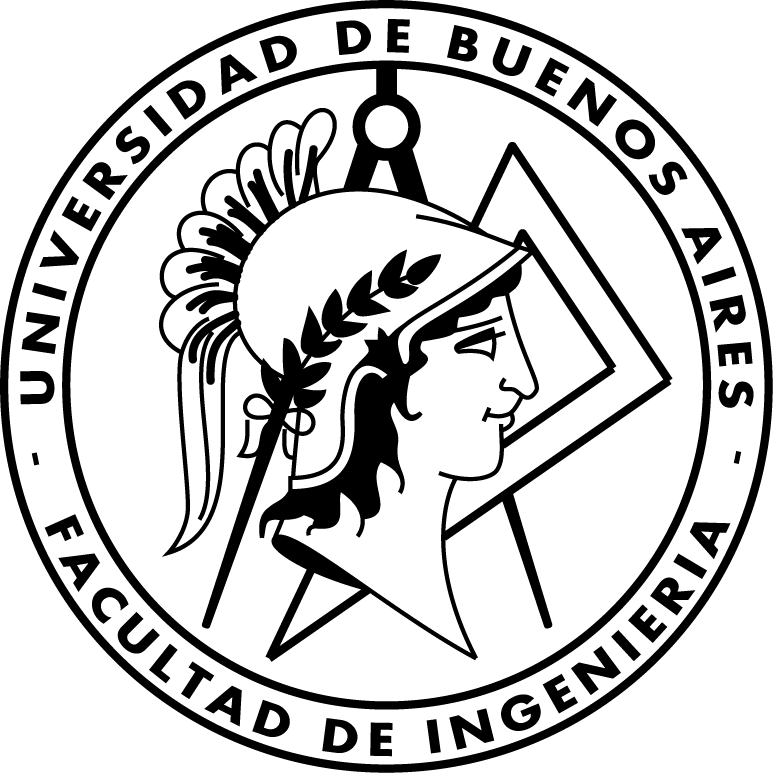
\includegraphics[width=0.25\textwidth]{Logo-fiuba.png}\\
%    \vspace{1cm}
%    {\bfseries \LARGE Facultad de Ingeniería}\\
%    \vspace{0.5cm}
%    {\scshape \Large Universidad de Buenos Aires}\\
%    \vspace{3cm}
%    {\scshape \Huge \thetitle}\\
%    \vspace{1cm}
%    {\scshape \Large \theclass}\\
%    \vfill
%    {\Large \theauthorJT}
%    \vfill
%    {\Large \thedate}
%\end{titlepage}

\begin{center}
	{\bfseries \LARGE \thetitle}
\end{center}

\noindent \textbf{Alumno:} Juan Ignacio Teich\\
\textbf{Director:} Dr. Alejandro Daniel Otero\\
\textbf{Co-Director:} Ing. Dimas Alejandro Barile\\
\textbf{Título:} \textit{\thesisname}\\

\textbf{\Large Descripción del tema}
\section{Resumen}
En este trabajo se realizará un análisis de los distintos modelos de actuadores discales disponibles en la bibliografía, variando parámetros característicos de cada actuador. Se analizará el comportamiento de los mismos frente a distintas condiciones, como puede ser estar detrás de la estela de otro actuador, ya sea interferencia parcial o total, distintos perfiles de velocidad de entrada, distinta orientación frente al viento, etc. Se evaluará la relación precisión-costo computacional de cada modelo contrastado contra la variante más exacta.


Este análisis permitirá una mejor selección del modelo adecuado para cada caso de aplicación considerando la mayor precisión posible al menor costo computacional.

\section{Estado actual del conocimiento sobre el Tema}
A la hora de simular aerogeneradores en parques eólicos, la representación exacta de los aerogeneradores resulta de un costo computacional muy elevado. Es por esto que se han desarrollado alternativas para poder simular su efecto, una de ellas siendo la técnica de actuadores. Entre ellos se encuentra el modelo de actuador discal \cite{mikkelsen_actuator_2004}. Este modelo consiste de un disco con fuerzas aplicadas sobre el fluido, equivalentes a las desarrolladas sobre las aspas de una turbina real. Al no necesitar incluir el detalle de las aspas, el costo computacional resultante es sumamente menor.

Dentro de los distintos modelos de actuadores discales se tiene una gama muy amplia de complejidad, dando resultados de variada satisfacción según el caso a simular. El modelo de actuador más preciso es el \textit{airfoil}, el cual incorpora la teoría del elemento de pala o perfil alar, desarrollando un disco con infinitos perfiles alares. El modelo más simple de actuador es el \textit{uniforme}, el cual distribuye de forma uniforme la fuerza del aerogenerador. Este modelo se encuentra muy limitado, solo pudiendo funcionar con velocidad uniforme a su entrada. Esto lo hace incapaz de simular diversos casos, como por ejemplo encontrarse en la estela de otro aerogenerador.

\section{Objetivos}
Como objetivo general de este plan de investigación se propone el desarrollo de un análisis paramétrico de los distintos actuadores discales disponibles en la bibliografía, comparando su comportamiento y costo computacional frente al actuador \textit{airfoil}.\\

\textbf{Objetivos específicos:}
\begin{itemize}
	\item Realizar una búsqueda bibliográfica sobre los actuadores discales disponibles y sus prestaciones.
	\item Implementar los actuadores discales a estudiar en el software OpenFOAM con condiciones de entrada de flujo uniforme y flujo atmosférico.
	\item Realizar simulaciones de un túnel de viento de todos los actuadores en situaciones de flujo libre, interferencia total o parcial.
	\item Analizar el costo computacional y la precisión obtenida en cada caso.
\end{itemize}

\section{Metodología y plan de trabajo}
El modelo CFD se realizará con el software open-source OpenFOAM, utilizándolo para resolver las ecuaciones de Navier-Stokes con simulaciones RANS (Reynolds Average Navier Stokes). Este software permite la implementación de los actuadores y el desarrollo de los casos necesarios para el análisis. Además, la simulación de los casos a desarrollar impone la necesidad de simulaciones en paralelo utilizando una gran cantidad de procesadores, para lo cual el software OpenFOAM es adecuado.

Se realizará un estudio bibliográfico de los actuadores desarrollados y además de características adicionales que puedan ser encendidas y apagadas al aplicar un aerogenerador. Luego se desarrollarán diversos casos de prueba tomados de la bibliografía, y se compararán los actuadores con el actuador \textit{airfoil}, el cual es aceptado como el más preciso en representar la realidad, aunque el de mayor costo computacional.

\section{Cronograma de tareas}
\begin{center}
\resizebox{\textwidth}{!}{\noindent
\begin{ganttchart}[
	canvas/.append style={fill=none, draw=black!5, line width=.75pt},
	hgrid style/.style={draw=black!5, line width=.75pt},
	vgrid={*1{draw=black!5, line width=.75pt}},
	title/.style={draw=none, fill=none},
	title label font=\bfseries\footnotesize,
	title label node/.append style={below=7pt},
	include title in canvas=false,
	bar label font=\mdseries\footnotesize\color{black},
	bar label node/.append style={left=2cm},
	bar/.append style={draw=none, fill=black!63},
	bar incomplete/.append style={fill=blue},
	bar progress label font=\mdseries\footnotesize\color{black!70},
	group incomplete/.append style={fill=blue},
	group left shift=0,
	group right shift=0,
	group height=.5,
	group peaks tip position=0,
	group label node/.append style={left=.6cm},
	group progress label font=\bfseries\small,
	]{1}{12}
	\gantttitle[
	title label node/.append style={below left=7pt and -3pt}
	]{Mes:\quad}{0}
	\gantttitlelist{1,...,12}{1} \\
	%\ganttgroup[]{Tesis}{1}{12} \\
	\ganttbar[
		bar/.append style={fill=blue},
		name=bar1
	]{\textbf{Capacitación en OpenFOAM}}{1}{2} \\
	\ganttbar[
		bar/.append style={fill=blue},
		name=bar2
	]{\textbf{Busqueda bibliográfica}}{3}{4} \\
	\ganttbar[
		bar/.append style={fill=blue},
		name=bar3
	]{\textbf{\parbox{6.5cm}{\begin{flushright}Desarrollo del modelo de túnel de viento con distintas condiciones de entrada y cantidad de aerogeneradores\end{flushright}}}}{5}{5} \\ 
	\ganttbar[
		bar/.append style={fill=blue},
		name=bar4
	]{\textbf{Simulaciones}}{6}{7} \\
	\ganttbar[
		bar/.append style={fill=blue},
		name=bar5
	]{\textbf{Análisis de resultados}}{8}{10} \\
	\ganttbar[
		bar/.append style={fill=blue},
		name=bar6
	]{\textbf{Redacción}}{11}{12} \\
	\ganttlink{bar1}{bar2}
	\ganttlink{bar2}{bar3}
	\ganttlink{bar3}{bar4}
	\ganttlink{bar4}{bar5}
	\ganttlink{bar5}{bar6}
\end{ganttchart}
}
\end{center}
%Referencias
\nocite{*}
\newpage
\printbibliography

\newpage
\noindent \textbf{Ámbito de desarrollo propuesto}\\
\indent Se propone como ámbito de trabajo el Centro de Simulación Computacional para Aplicaciones Tecnológicas (CSC, CONICET).\\

\noindent  \textbf{Aval de Director, Co-Director y CV}\\
\indent Se adjuntan los documentos.\\

\noindent \textbf{Estimación de costos y la previsión de la fuente de financiamiento}\\
\indent El Centro de Simulación Computacional para Aplicaciones Tecnológicas cuenta con computadoras disponibles para realizar las simulaciones necesarias.\\

\noindent \textbf{Solicitud de Alta de TIM}\\
\indent Sirva la presente propuesta de Tesis de Ingeniería Mecánica como solicitud formal de alta.\\

\noindent  \textbf{Acta de acuerdo entre Director, Co-Director y Alumno}\\
\indent Se adjuntan el documento.\\

\end{document}
